\section{Introduction}

\subsection{Motivation: background of the problem of image matting algorithms}
\label{sec:motivation}
The evolution and usage of Image-Matting algorithms have increased in popularity. The precise extraction of foreground objects is used in image and video editing. It also has several important uses in entertainment, advertising, and e-commerce. It is used for special effects where the foreground needs to be identified. Many e-commerce shops use it indirectly to create a clean look for their products by cutting out the background so that the focus remains on the product. 
image-matting algorithms allow us to separate foreground and background precisely.

The challenge in image-matting algorithms lies in finding a reliable and efficient method to determine how much each pixel belongs to the foreground or background. Traditional manual segmentation methods, for example, choosing the pixel with your brush tool on your own, while accurate, is time-consuming and not scalable for larger datasets. This is where image-matting comes in, aiming to simplify the process. However, these algorithms, like the ones that you will get introduced to later, are not without challenges. They struggle with accurately capturing fine details and textures, dealing with half-transparency, and managing complex scenarios with multiple objects.

Two well-known methods are K-Nearest-Neighbor-Matting (KNNM) and Closed-Form-Matting (CFM). 
K-Nearest-Neighbor-Matting \citep{knn}  tries to use K-Nearest-Neighbor to identify the k pixels that are similar to each pixel. The publishers promise fast and precise foreground separation at holes and complex regions. Nevertheless, it tends to be less precise in smooth areas.
Closed-Form-Matting \citep{cf} uses something that is called color line assumption (color line model). The publishers promise fast and precise foreground separation in smooth areas. Still, it has also been shown to be less precise at holes and complex regions. 

\begin{figure*}[t!]
	\centering
	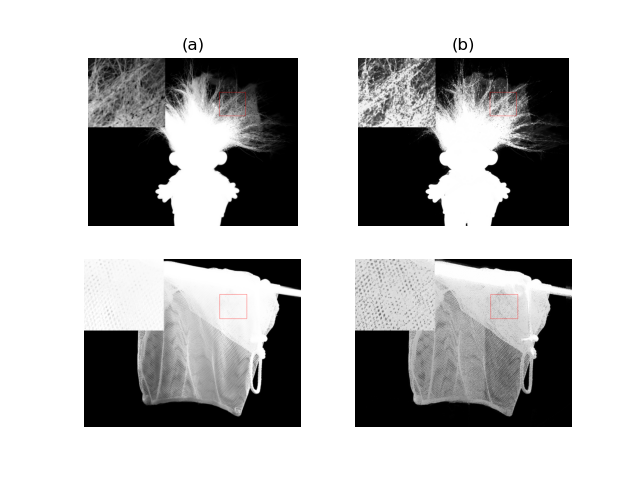
\includegraphics[]{bilder/cfknnvergleich}
	\caption{Difference between KNNM and CFM: (a) CFM and (b) KNNM.}\label{fig_cf_knn}
\end{figure*}


In this bachelor thesis, we will examine the background and motivation behind Image-Mapping algorithms, also called Alpha-Matting algorithms. We will implement an algorithm, show its experimental results, and draw a conclusion based on its results.
\subsection{Goal: What does the mentioned algorithm try to do} 

In this thesis, we aim to build an efficient method that solves the problems that both the KNNM and the CFM had before. This method should be able to separate precisely the foreground from the background in areas like holes, complex regions, and smooth areas. 

Therefore, we will be implementing the algorithm \citep{lnclm} from the paper "Local and Nonlocal Color Line Models for Image Matting" which tries to combine the CFM algorithm with the KNNM algorithm. The algorithm will be called LNCLM algorithm.


\section{Foundations}
In this section, we will learn all the necessary methods to understand the algorithm from the paper "Local and Nonlocal Color Line Models for Image Matting". We will also understand how these foundations connect to the algorithm described. 

\subsection{Trimap}
A Trimap is separated in 3 regions. The foreground, background and unknown. It is usually used in Alpha-matting algorithms and we will use it as a second input for the LNCLM algorithm. It usually created by the user of the algorithm.
The foreground region is marked in white and covers the pixels that definitely belong to the foreground.
The background region is marked in black and covers the pixels that definitely belong to the background.
The unknown Region is marked in gray and covers the pixels where the user is unsure if it belongs to the background or foreground.

\begin{figure}[htb]
	\begin{center}
		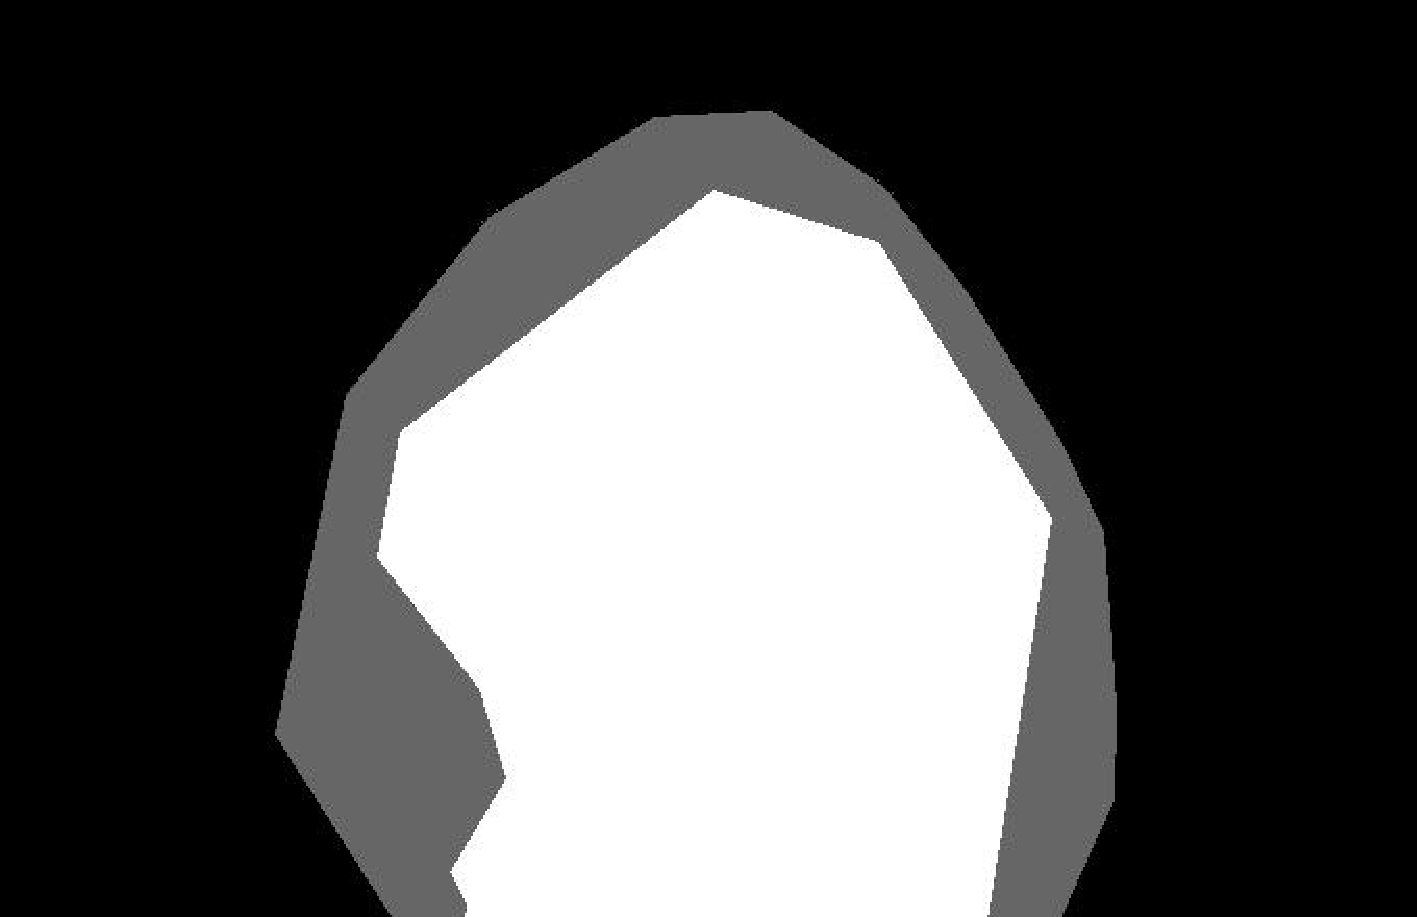
\includegraphics[width=175pt]{bilder/trimap}
		\caption{Example of a trimap}\label{fig_trimap}
	\end{center}
\end{figure}

The Trimap's quality directly impacts the precision of the resulting segmentation. Subsequently, the Alpha-Matting algorithm takes the lead, employing various techniques, like for example kNN or the local color line model, to discern the identity and extent of the unknown pixels, whether they belong to the foreground or background. 

\subsection{Local color line model}
\label{sec:localcolor}
The Local color line model is a fundamental concept in the LNCLM algorithm. It posits that the pixels residing between the foreground and background of an image form a distinct color line in the RGB 3D space.
To understand this further, we need to understand that the colors are not chosen randomly between the background and foreground. Furthermore, they tend to follow certain patterns and trends. These patterns can be visualized as color lines in color space. 
Therefore, we can write two similar formulas.
\begin{align}\label{eq_f}
	F_{i} = \beta_{i}^{F}F_{1} + (1 - \beta_{i}^{F})F_{2}   
\end{align}
\begin{align}\label{eq_b}
	B_{i} = \beta_{i}^{B}B_{1} + (1 - \beta_{i}^{B})B_{2}   
\end{align}

The variables \(F_1\) and \(F_2\) stand for two different pixel in the foreground and \(B_1\) and  \(B_2\) stand for two different pixel in the background. If we imagine a straight line going from one to two, then  \(\beta_i\) is defined as between  \([0;1]\) and stands for how near we go from pixel one to two. Here, we can see it visualized in Figure (\ref{fig_formel}).

\begin{figure}[htb]
	\begin{center}
		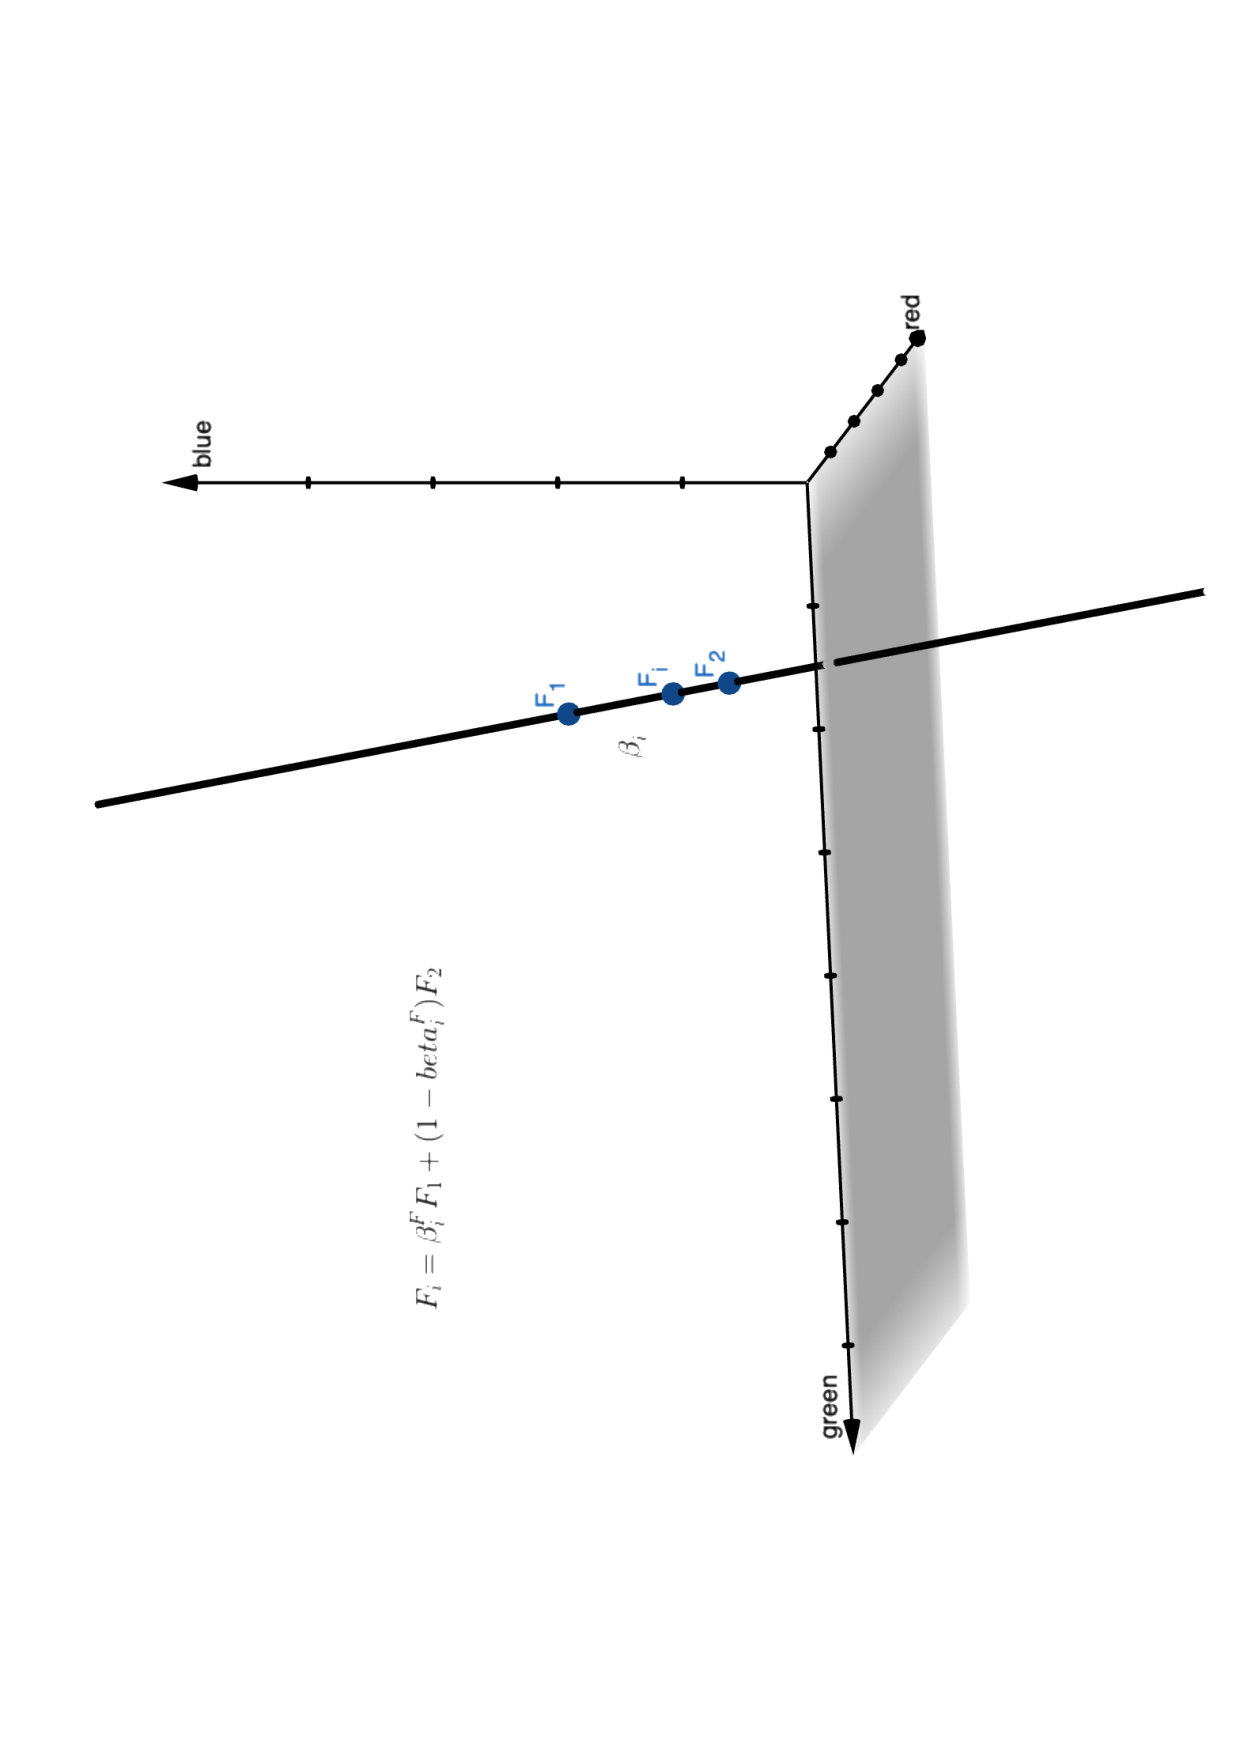
\includegraphics[width=300pt, angle=270]{bilder/formel}
		\caption{Pictorial example of the formula}\label{fig_formel}
	\end{center}
\end{figure}

\subsection{K-Nearest-Neighbours}
The K-Nearest-Neighbours method is generally based on the concept of neighborhood, where the majority of its nearest neighbors determine the class assignment of an unknown observation. The parameter k determines the number of nearest neighbors used for classification. One crucial aspect of K-Nearest-Neighbours is that the algorithm learns from the existing training data and uses this information to classify new, unknown data. This flexibility makes the kNN classifier exceptionally versatile and adaptable to different types of data and problems \citep{knearestneighbour}. 
This is the general use case of K-Nearest-Neighbours. However, the KNNM and LNCLM algorithms are used differently. Instead of classification, we only want to know the neighbors of a specific pixel. For example, if our k is 20 and the pixel of our choice is a random pixel, we want to know which 20 pixels are the closest to this random pixel. Nearest in the context of Image-Matting means a similar appearance and spatial nearest \citep{lnclm}.

\begin{figure}[htb]
	\begin{center}
		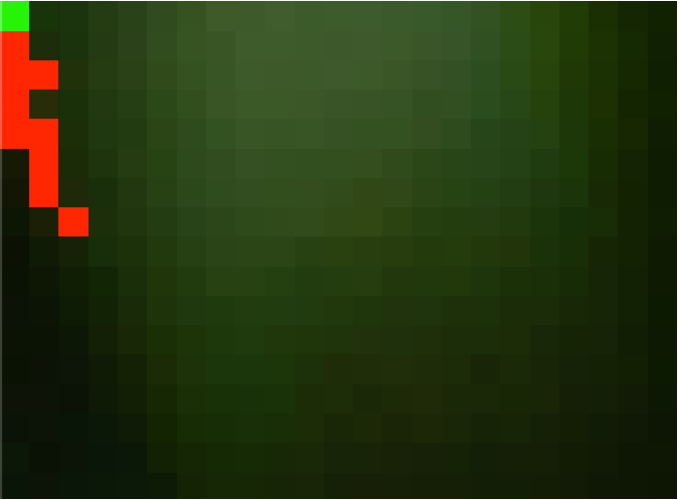
\includegraphics[width=200pt]{bilder/knn}
		\caption{Example for KNN}\label{fig_knn}
		\medskip
		\small{If we choose k = 10 and want to search for the k-Nearest-Neighbor for the green pixel, then the red ones are the neighbors}
	\end{center}
\end{figure}



\subsection{Difference: Local Nonlocal Neighbors}
The difference between Local and Nonlocal Neighbors lies in the selection of the neighbors. The local neighbors are the pixels that sit around a specific pixel in a window (\ref{fig_ColorLineModel}). This approach is used in CFM.
The Nonlocal Neighbors are pixels that look similar to the pixel we are looking at (\ref{fig_knn}). This approach is used in KNN-Matting.
These neighbors should share the same alpha-values as the pixels looked at. Both approaches are later used in the LNCLM algorithm. \cite{lnclm}


\section{Related Work}
In this section, we will learn the related works that will help us further comprehend the LNCLM algorithm. We will also understand how these related works connect to the described algorithm (\hyperref[sec:algorithm]{section: LNCLM algorithm}).
\subsection{Closed-Form-Matting}
\label{sec:closedform}
CFM aims to find the optimal alpha matte by minimizing a cost function that shows the difference between the estimated alpha value and the ground truth alpha value of all pixels in the image based on the color line model.
Let us go through the steps together to understand the derivation of the cost function in closed-form matting.
First of all, we will learn about the matting equation: 
\begin{align} \label{eq:3}
	I_i  = \alpha_iF_i + (1-\alpha_i)B_i . 
\end{align} 
The variable \(I_i\) is the color value of the \(i\)th pixel while \(F_i\) and \(B_i\) are the foreground and background color values of the \(i\)th pixel. The variable \(\alpha_i\) has the range [0,1] and stands for the foreground opacity \cite{cf}. This equation is the basis of the matting problem, where the goal is to get a near approximation of the absolute \(\alpha\).

The color line model(\hyperref[sec:localcolor]{subsection: Local color line model}) assumes that the pixels of the background and foreground over a small window are approximately constant. Because of this assumption, we can build this equation: 
\begin{align}  \label{eq:4}
	\alpha_i \approx a I_i + b .
\end{align}
While a is the gradient or slope of this linear function, and it is defined in \cite{cf} as
\begin{align}
	a  = \frac{1}{F-B}
\end{align}  
and b is seen as the y-intercept and is defined in \cite{cf} as
\begin{align}
	b  = -\frac{B}{F-B}.
\end{align}  

Now, for the first time, we will define the cost function. We will start by defining it over a window \(w_j\) around each pixel j: 
\begin{align}
	J(\alpha, a, b) = \sum_{j} \sum_{i \in w_j} (\alpha_i - a_j I_i - b_j)^2 + \epsilon a^2_j .
\end{align}  
The second term \(\epsilon a^2_j \) is an error term to ensure numerical stability. The goal is that \(\alpha_i - a_j I_i - b_j)^2 \) this term will be zero for every pixel and this is how the equation is going to be reformulated: 
\begin{align}
	(a_j, b_j) = \text{argmin}_{a,b} \sum_{i \in w_j} (\alpha_i - a I_i - b)^2 + \epsilon a^2
\end{align}  

By solving this minimization problem, we can reformulate the function again:
\begin{align}
	J(\alpha, a, b) = \sum_k || G_k \begin{pmatrix} a_k \\ b_k \end{pmatrix} - \alpha_k ||^2 .
\end{align}  
The variable \(G_k \) is a matrix that contains the color information of the window k, and \(\alpha_k\) is a vector of \(\alpha\)values. The optimal a and b are now given by 
\begin{align}
	\begin{pmatrix} a_k \\ b_k \end{pmatrix}  = \left( G_k^T G_k\right)^{-1} G_k^T \alpha_k  
\end{align}  
Substituting the optimal a and b back into the cost function, we get this form:
\begin{align}
	J(\alpha) = \sum_{k} \bar{\alpha}_k^T \bar{G}_k^T \bar{G}_k \bar{\alpha}_k
\end{align}  
The variable \(\bar{G}_k\) is defined as \( I - G_k(G_k^T G_k)^{-1} G_k^T\)
Moreover, \(\bar{G}_k^T \bar{G}_k\), which will later be the Laplacian matrix \(L\), is an \(N \times N\) matrix whose (i,j)-th entry is:
\begin{align} \label{eq:12}
	L_{ij} = \sum_{k | (i,j) \in w_k} \left( \delta_{ij} - \frac{1}{|w_k|} ( 1 + (I_i - \mu_k)(\sigma_k + \frac{\epsilon}{|w_k|} I_3)^{-1}(I_j - \mu_k) )  \right) 
\end{align}  
The variable \(\delta_{ij}\) is the Kronecker delta, \(\sigma_k\) and \(I_3\) are  \(3 \times 3\) covariance and identity matrices, and \(\mu_k\) is a \(3 \times 1\) mean vector of the colors in the k-th window.

After we changed the cost function, we extended the linear model \ref{eq:4} to include all color channels separately: 
\begin{align}\label{eq:13}
	\alpha_i \approx \sum_{c} a_c I_{ic} + b .
\end{align}  

When we now fuse \ref{eq:12} and \ref{eq:13}. Therefore, we get this quadratic form:
\begin{align}
	J(\alpha) = \alpha^T L \alpha
\end{align}  

Finally, to find the optimal alpha matte, we equate the cost function to 0 like this:
\begin{align}
	0 =  L \alpha
\end{align}  


Compared to LNCLM, CFM only uses local neighbors, while LNCLM also uses non-local neighbors. The CFM algorithm searches consider the pixels around each pixel, which further leads to smooth segmentations where there should be harsh ones. The LNCLM uses the k nearest pixels and leads to more precise $\alpha$-values in holes and complex areas. 




\subsection{KNN-Matting}
The Goal of KNNM is to find the optimal alpha matte by minimizing a cost function that shows the difference between the estimated alpha value and the ground-truth alpha value of all pixels in the image based on k nearest neighbours.
Let us go through the steps together to understand the derivation of the cost function in KNNM.

First of all, the Laplacian matrix is defined \cite{knn}:
\begin{align}
	L = D - A .
\end{align}
The variable D is an N × N diagonal matrix, where N is the total number of pixels, and A is the nonlocal affinities matrix. The nonlocal affinities matrix shows us how \cite{knn} is defined as: 
\begin{align}
	A & = [k(i,j)]\\
	k(i,j) & = \text{exp}(- \frac{1}{h_1^2} || X(i) - X(j) ||^2_g - \frac{1}{h_2^2} d_{ij}^2) .
\end{align}
For better understanding, we choose pixels i and j are the pixels most similar to those chosen by k nearest neighbor. The feature vectors X(i) and X(j) are computed at pixel i or j. The constants \(h_1\) and \(h_2\) are found by trying, \(d_ij\) is the distance between the pixels i and j, and \(|| \cdot ||_g\) is a norm weighted by a center-weighted Gaussian.

Now the cost function gets introduced \cite{knn}:
\begin{align}
	g(x) = x^T L x + \lambda \sum_{i \in m - v} x_i^2 + \lambda \sum_{i \in v} (x_i - 1)^2
\end{align}
Just to clarify \(J\), from (\hyperref[sec:closedform]{subsection: Closed-Form-Matting}), and \(g\) stand both for cost function and \(x\) stands for  \(\alpha\). The term \(\lambda \sum_{i \in m - v} x_i^2\) handles the unmarked pixels and \(\lambda \sum_{i \in v} (x_i - 1)^2\) ensures that marked pixels are close to their specified values. 

The cost function gets reformulated and put into the matrix form:
\begin{align}
	g(x) & = x^T L x + \lambda \sum_{i \in m} x_i^2 - 2 \lambda v^T x + \lambda |v|\\
	& = \frac{1}{2}x^T 2 (L + \lambda D) x - 2 \lambda v^T x + \lambda |v|
\end{align}
The vector \(v\) is a binary vector for the marked pixels.

Through deriving and equating the cost function with zero, we get the optimal alpha matte:
\begin{align}
	x = (L + \lambda D)^{-1}(\lambda v)
\end{align}

Compared to LNCLM, KNNM only uses non-local neighbors, while LNCLM also uses local neighbors. The KNNM algorithm searches for the k nearest pixels for each pixel based on color and spatial information, which does not include any smoothness assumption, which further leads to harsher segmentations. This is compared to LNCLM, which also uses a local window around each pixel and therefore, leads to more precise $\alpha$-values in smooth and complex areas. 






\section{Methods of Evaluation}
In this section, we will learn some evaluation methods to evaluate the algorithm from the paper "Local and Nonlocal Color Line Models for Image Matting." 

\subsection{MSE}
The mean squared error is a risk function that uses quadratic loss  \cite[p.\ 20]{mse}. It calculates the squared differences between observed and estimated values. The formula for MSE is 

\begin{align}
	\text{MSE}( \hat{\theta} ) = \mathbb{E}[ ( \hat{\theta} - \theta)^2 ]. 
\end{align}
Where \(\hat{\theta} \) is the estimator of \(\theta\).
For our practical calculations, we use a transformation of the formula \cite{lnclm}: 
\begin{align}
	\text{MSE}(\alpha^*) = \left(  \frac{\sum_i \left( \alpha_i - \alpha^*_i \right)^2}{N_{\text{unk}}}  \right) .
\end{align} 
Where \(\alpha^*\) are the predictions of the \(\alpha\) values. The variable \(N_{\text{unk}}\) is the number of pixels in the unknown region of the Trimap. In this derivation of the function, we go through all the \(\alpha\) values and subtract the predicted alpha value from our true alpha value, also called ground truth, which then gets squared and divided by the number of unknown pixels. A low MSE indicates better performance because the model's predictions are highly accurate and closely match the actual observed values. A high MSE suggests bad performance because the model's predictions are not accurate and does not closely match the actual observed values. The MSE helps us compare the different alpha matting methods and identify the one with the most accurate alpha value estimations. It is also one of two evaluation metrics in the paper \cite{lnclm} to compare the LNCLM algorithm. 

\subsection{SAD}
The sum of all differences is another evaluation metric. It calculates the differences between observed and estimated values. The formula for SAD is
\begin{align}
	\text{SAD} = \sum_{i=1}^m \sum_{j=1}^n |A(i,j) - B(i,j)|. 
\end{align}
The variables \(A(i,j)\) and \(B(i,j)\) are the pixels at position \((i,j)\) in image \(A\) and \(B\). The constants \(m\) and \(n\) are the height and width of these images.  
For our practical calculations, we use a derivation of the formula \cite{lnclm}:
\begin{align}
	\text{SAD}(\alpha^*) = \sum_i |\alpha_i - \alpha^*_i| .
\end{align} 

Where \(\alpha^*\) are the predictions of the \(\alpha\) values. In this derivation of the function, we go through all the \(\alpha\) values and subtract the predicted alpha value from our true alpha value. A low SAD indicates better performance and a high SAD suggests bad performance. The SAD also helps us compare the different alpha matting methods and identify the one with the most accurate alpha value estimations. It is the second evaluation metric in the paper \cite{lnclm} to compare the LNCLM algorithm. 

\subsection{Dataset for evaluation}
We used alphamatting.com as a dataset to evaluate our code. It was first proposed in a paper \cite{benchmark} and was meant to be the first standard library for image matting algorithms to be tested. Already existing datasets to that point were affected by noise, which refers to random pixels that do not represent the actual scene. Also, they were primarily biased towards specific algorithms. One had, for example, more smooth images, which would favor algorithms like CFM, and others had more images with hard segmentations, which would favor algorithms like KNNM. Most old datasets had high-quality images, though they included artificial backgrounds and lacked diversity.
The improved dataset \cite{benchmark} is augmented with natural scenes, diverse focus settings, and translucent objects. It provides data, scripts for community contributions, and enables interactive analysis of new results. Most importantly, the new dataset reveals the weaknesses and strengths of matting algorithms so we can reliably compare our LNCLM algorithm with others.



\section{LNCLM algorithm}
\label{sec:algorithm}
In this section, we will learn the algorithm proposed in the paper "Local and Nonlocal Color Line Models for Image Matting" \cite{lnclm}. It segments the foreground from the background, and we will especially have a look at the Nearest Neighbour color line model. 

\subsection{Introduction into the Nearest Neighbour color line model}
As already mentioned in (\hyperref[sec:motivation]{section: Motivation}), the CFM tends to be very precise in smooth areas, for example, with fur, but unprecise in complex areas, for example, with nets and glass. Meanwhile, the KNNM tends to be the complete opposite. It is exact in complex areas and very imprecise in smooth areas.
That is why the authors wanted a color line model that combined the benefits of both Matting algorithms. This resulted in the Nearest Neighbour color line model.
The premise of the Nearest Neighbour color line model, short NNCLM, is that the nearest neighbors of the feature vectors follow the color line model. The feature vector will be explained in the following subsection.

\subsection{Feature Vector}
\label{subsec:feat}
The feature vectors represent each pixel in multidimensional space and include spatial and color information. This helps to find the nearest neighbor to each pixel. The feature vector proposed in the paper \cite{lnclm} is
\begin{align}
	X(i) = (I^r,I^g,I^b,x,y)_i .
\end{align} 
The variable i stands for the pixel i. The values \(I^r\), \(I^g\), and \(I^b\) stand for the RGB color information that the pixel I contains. While \(x\) and \(y\) represent spatial information. In our implementation of LNCLM, we weight the spatial coordinates with dws to make them less important. 


\begin{algorithm}
	\begin{algorithmic}[1]
		
		\State $ f = [I_r, I_g, I_b, \text{dws} \cdot x,   \text{dws} \cdot y ]$
		
	\end{algorithmic}
\end{algorithm}

The distance between two pixels is called the Euclidean distance and is calculated like this: 
\begin{align}
	\text{Euclidean distance} = ||X(i) - X(j)|| . 
\end{align} 
This is used to find the nearest neighbors through K-Nearest-Neighbor.



\subsection{NN-Color-line Derivation}
\label{nncolor}
The assumption is that the NNCLM and the KNN follow the color-line model. Figure 6 shows that the assumption is valid for smooth and complex regions. You can see the linear distribution of KNN foreground and background. 

\begin{figure}[htb]
	\begin{center}
		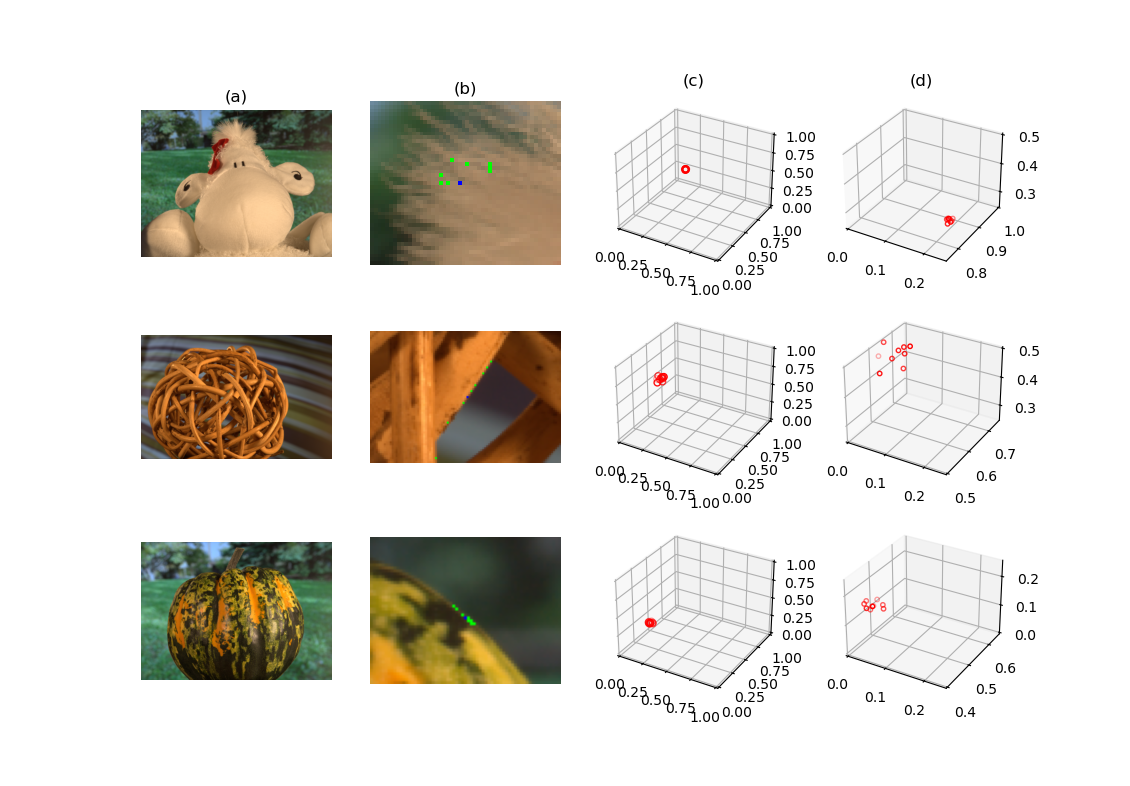
\includegraphics[width=400pt]{bilder/clm}
		\caption{Examples showing that KNN satisfies the color line model (K = 9).
			(a) original images, (b) zoomed-in images. The green pixel\textit{} (marked) are the KNN of the blue pixel (also marked). (c) foreground and background color distributions of the KNN in (b), respectively. (d) zooms into (c).}\label{fig_knn_in_action}
	\end{center}
\end{figure}

However, this does not mean that the feature vectors are linearly aligned, but the color components are. 
Because of that, the foreground and background can be represented by convex functions(\ref{eq_f}) and (\ref{eq_b}).
The value \( N_i\) represents the neighbor vectors for a specific pixel i. The variables \(F_1\), \(F_2\), \(B_1\), and \(B_2\) are constant colors over \(N_i\) (\ref{fig_ColorLineModel}) . As we already explained in (\hyperref[sec:localcolor]{section: Local color line model}). This formula and the matting equation used in CFM (\ref{eq:3}) can be combined. Therefore, the pixel for all j in \(N_i\) can be described as
\begin{align}
	I_j = \alpha_j(\beta_{j}^F F_1 + (1 - \beta_{j}^F)F_2) + (1- \alpha_j)(\beta_{j}^B B_1 + (1-\beta_{j}^B)B_2), \forall j \in N_i .
\end{align} 
We can obtain a 4D model out of this formula, as in CFM 
\begin{align} \label{eq:14}
	\alpha_j = a_i^R I_j^R + a_i^G I_j^G + a_i^B I_j^B + b_i, \forall j \in N_i .
\end{align} 
The variables \(I_j^R\), \(I_j^G\), and \(I_j^B\) are the red, green, and blue values of the \(j\)th pixel. While \(a_i^R\), \(a_i^G\), and \(a_i^B\) are the gradients or slope of this polynomial function and they are defined in \cite{cf} as
\begin{align}
	a  = \frac{1}{F-B}.
\end{align}  
and b is seen as the y-intercept and is defined in \cite{cf} as
\begin{align}
	b  = -\frac{B}{F-B}.
\end{align}  

\subsection{Cost Function from NN-Color-line-model}
The 4d model (\ref{eq:14}) can be denoted to this cost function
\begin{align}
	J_n = \sum\limits_{i\in I} \left( \sum\limits_{j \in N_i} \left( a_j -\sum\limits_{C} a_i^C I_j^C - b_i \right) ^2 + \epsilon\sum\limits_{C} \left( a_i^C \right) ^2 \right).
\end{align} 
The variable \(I^C\) is the entire image, C is the different color channels, and \(\epsilon\) is a constant for regularization. The cost function has \(5N\) unknowns and \(\alpha\), \(a_i^C\), and \(b_i\) are quadratic. The variables \(a_i^C\) and \(b_i\) can be eliminated by Theorem 2 in \cite{cf}. Which reduces the cost function to only depend on \(\alpha\). Now, the formula can be rewritten into
\begin{align}
	J_n = \alpha^T L_n \alpha .
\end{align} 
The variable \(\alpha\) is an \( N \times 1 \) vector, and \(L_n\) is an \(N \times N\) Laplacian matrix. The \( (j,k) \)th element of the Laplacian matrix \(L_n\) is 
\begin{align}\label{eq:37}
	\sum_{i|(j,k) \in N_i} \left( \delta_{jk} - \frac{1}{|N_i|} \left(1+ \left( I_j - \mu_i \right)^T \left( \Sigma_{i} + \frac{\epsilon}{|N_i|} I_3 \right)^{-1} \left( I_k - \mu_i \right) \right) \right) .
\end{align} 
The variable \(\delta_{jk}\) is the Kroenecker delta, which is one if j is equal to k else it is 0. The variable \(\Sigma_i\) is a three-by-three covariance matrix, which contains the covariances of the three color channels, \(\mu_i\) is the mean vector of the three color channels, and \(I_3\) is a three by three Identity matrix.
The intuition behind the simplification is that by eliminating  \(a_i^C\) and \(b_i\), the cost function \(J_n\) becomes a quadratic form in terms of a. This simplification minimizes the quadratic form and using linear algebra methods we can find the alpha values. The Laplacian matrix \(L_n\) contains the relationship between each pixel and each other, considering both color information and spatial relationships within neighborhoods \(N_i\).

Because of this cost function, we now have several advantages. Due to the nonlocal principle, the LNCLM is effective across different images with color variations. Also, by considering all color variations, the LNCLM can reflect foreground and background variations more accurately, leading to more accurate alpha mattes. Therefore, the LNCLM  performs better in images with a lot of color variation, for example, with fur. It overcomes the limitations of previous methods by not solely relying on appearance similarity. Nevertheless, it still needs improvement.  


\subsection{Combining Nearest Neighbors Color Line Model with Local Color Line Model}

The authors now combine the cost functions of the Nearest-Neighbors color line model and the local color line model
\begin{align}
	J & = \mu J_n + (1 - \mu) J_l + \lambda(\alpha^T - b^T_S )D_S(\alpha - b_S)\\ 
	& = \mu \alpha^T L_n \alpha + (1 - \mu)\alpha^T L_l \alpha + \lambda(\alpha^T - b_S^T)D_S(\alpha - b_S) .
\end{align} 
The constant \(\mu\) balances the cost functions between the local and NN color line models. While \(\lambda\) is a large number for the smoothness term. The diagonal matrix \(D_S\) indicates a constrained pixels. Also, the vector \(b_S\) contains specified alpha values for the constrained pixels. 

The reason for that is that NNCLM is not as smooth as anticipated. This leads us also to apply the local color line model to the image. Now, we have the results of the NNCLM and the local color line model, which can now be fused. Only applying one will lead us to either too segmented rough of an $\alpha$ matte or too smooth.

By calculating the maximum of \(J\), through differentiating the cost function and setting the derivatives to zero, we get this function: 
\begin{align}\label{eq:40}
	\alpha = (\mu L_n + (1 - \mu) L_l + \lambda D_S)^{-1} \lambda b_S .
\end{align} 



\section{Implementation}
With our newly acquired theoretical knowledge, we are now ready to apply the LNCLM algorithm in practical scenarios.

\subsection{Basic Implementation}
This subsection will provide a comprehensive overview and a detailed understanding of the LNCLM algorithm structure, equipping us with in-depth knowledge that will be further expanded in the subsequent sections.
Like most alpha matting algorithms, the LNCLM algorithm gets an image and a Trimap as input. These inputs are used to calculate the cost function, resulting in us getting our alpha matte. 
This alpha matte can then be applied via the matting equation \ref{eq:3} to get our foreground and background. The now shown pseudo code will clarify this further:

\begin{algorithm}
	\caption{LNCLM Algorithm}\label{lnclm}
	\begin{algorithmic}[1]
		\State $\textbf{Input: }  \text{image and trimap}$ 
		\State $\textbf{Output: }  \text{alpha matte}$
		\newline
		\State $\text{neighborsnnclm} \gets \text{the neighbors for each pixel calculated by kNN} $
		\State $\text{neighborscf} \gets \text{the neighbors for each pixel in a window} $
		\newline
		\State $ \text{\(L_n \)} \gets \text{calculated Laplacian matrix with neighborsnnclm as input}$
		\State $  \text{\(L_l\)}  \gets \text{calculated Laplacian matrix with neighborscf as input}$
		\newline
		\State $ \text{\(\alpha\)} \gets \text{calculated alpha matte with \(L_n\) and \(L_l\) as input}$
		\State $\textbf{return} \text{ \(\alpha\)}$
	\end{algorithmic}
\end{algorithm}

The variable neighborsnnclm contains the neighbors to every pixel in the image. They are calculated by kNN, similarly to neighborscf, which contains the neighbors to every pixel. These neighbors are simply just the pixels that are in the window area of the chosen pixel. 
Both \(L_n\) and \(L_l\) are both Laplacian matrices, which are calculated with the neighbors as input and are calculated by this formula \ref{eq:37}. 
The \(\alpha\)-value gets \(L_n\) as well as \(L_l\) as input and solves this equation (\ref{eq:40}).


\subsection{Finding the Neighbors}
\label{subsec:neigh}
In this subsection, we will learn how to find the neighbors for the NNCLM and CFM parts of the LNCLM Algorithm. 

The explanation is based on this pseudo-code: 

\begin{algorithm}
	\caption{Searching for neighborsnnclm}\label{neighborsnnclm}
	\begin{algorithmic}[1]
		\State $\textbf{Input: }  \text{image, dws, nn}$
		\State $\textbf{Output: }  \text{neighborsnnclm}$
		\newline
		\State $\text{h, w} \gets \text{image.shape} $
		\State $\text{r, g, b} \gets \text{image.colors} $
		\newline
		\State $\text{x, y} \gets \text{Coordinates for every pixel} $
		\newline
		\State $ \text{f} \gets \text{\([r, g, b, \text{dws} \cdot x,   \text{dws} \cdot y]\) }$
		\State $  \text{neighborsnnclm}  \gets \text{knn(f, nn)}$
		\newline
		\Return $ \text{ neighborsnnlcm}$
	\end{algorithmic}
\end{algorithm}

As input we get the image, dws, and nn. The variable dws is weights the spatial coordinates of each pixel. The variable nn lets us decide how many neighbors we want to get for each pixel. In \cite{lnclm} dws is 0.5 and nn is 9.
In lines 3 and 4, we get the height, width, and RGB color information of the image. Afterward, we build a coordinate system so that we can associate every pixel with a spatial coordinate. The values r, g, b, x, and y now get passed into the feature vector, which we explained beforehand in (\hyperref[subsec:feat]{subsection: Feature Vector}).
The feature vector now gets used by knn, which lets us find our nearest neighbors based on the feature vector. We use FLANN like in \cite{lnclm}, an easy and fast way to implement kNN. These neighbors now get returned.


Now to searching neighborscf:
\begin{algorithm}[t]
	\caption{Searching for neighborscf}\label{neighborscf}
	\begin{algorithmic}[1]
		\State $\textbf{Input: }  \text{image, radius}$
		\State $\textbf{Output: }  \text{neighborscf}$
		\newline
		\State $\text{h, w} \gets \text{image.shape} $
		\newline
		\For{$\text{i = radius to h - radius}$}
		\For{$\text{j = radius to w - radius}$}
		\State $\text{Add the pixels in the window around pixel ij to neighborscf}$
		\EndFor
		\EndFor
		\newline
		\Return $\text{ neighborscf}$
	\end{algorithmic}
\end{algorithm}

The radius is the radius of the window around pixel ij. In \cite{lnclm}, it is 1.
Finding the neighbors for neighborscf is as easy as explained before. We go through each pixel of an image and put the neighboring pixels around the pixel ij into neighborscf. The only obstacle is the pixel at the edge of the image because they can not have a window of neighbors without exceeding the edge of the image. That is why we exclude them in the loops. 

To make this part faster, we used njit from numba. A compiler speeds up our code by generating optimized machine code. We also used numba.prange to parallelize the nested for loops. 

\subsection{Calculating the Laplacian Matrix}
\label{subsec:laplace}
The Laplacian matrix is calculated using the formula (\ref{eq:37}). The code shown now works out the formula in practice. 

\begin{algorithm}[t]
	\caption{Calculating the Laplacian matrix}\label{laplace}
	\begin{algorithmic}[1]
		\State $\textbf{Input: }  \text{image, trimap, neighbors }$
		\State $\textbf{Output: }  \text{Laplacian matrix L}$
		\State $\text{Initialize \(i\), \(j\), and \(v\) as arrays}$
		\State $\text{known} \gets \text{load all known pixels from trimap}$
		\For{$\text{pixels \(\in\) image}$}
		\State $\text{nn} \gets \text{load neighbors for this pixels}$
		\newline
		\If{nn are all known} 
		\State $\text{continue}$
		\EndIf
		\newline
		\For{$\text{dc in range(3)}$}
		\State $\text{\(\mu_i\)} \gets \text{mean of nn in every color channel}$
		\EndFor
		\newline
		\State $c \gets \text{nn} - \mu$
		\State $\text{cov} \gets \text{covariance matrix of \(c\)}$
		\State $\text{covtmp} \gets \text{cov + (\( \epsilon / \) nn.length ) *  \(I_3\)}$
		\State $\text{inv} \gets \text{invert covtmp}$
		\newline
		\For{$\text{di \(\in\) nn}$}
		\For{$\text{dj \(\in\) nn}$}
		\State $\text{Add spatial coordinates of di to \(i\)} $
		\State $\text{Add spatial coordinates of dj to \(j\)} $
		\newline
		\State $\text{tmp} \gets \text{c[di].dot(inv).dot(c[dj])}$
		\newline
		\If{i == j}
		\State $\text{tmp} \gets \text{1.0 - (1 + tmp) / nn.length} $
		\Else $\text{ tmp} \gets \text{0.0 - (1 + tmp) / nn.length} $
		\EndIf
		\State $\text{Add tmp to \(v\)}$
		\EndFor
		\EndFor
		\EndFor
		\State $ L \gets \text{Build matrix L with the values \(v\) at the coordinates \((i, j)\)}$
		\Return $L$
	\end{algorithmic}
\end{algorithm}

The Inputs are the image, trimap, and either neighborscf or neighborsnnclm because this method gets used twice, once with neighborscf and another time with neighborsnnclm. We initialize the arrays i, j, v, and load all known pixels from the trimap. Which are the pixels outside of the unknown region. 
Afterward, we start a for loop in which we go through every pixel in the image. In every iteration, we load the neighbors of the now chosen pixel. If these pixels are outside of the unknown region, so known then we skip this iteration because \(\alpha\) value is either 0 or 1. We now calculate the \(\mu_i\) of every neighbor in every color channel. We now calculate in \ref{eq:37} the terms \(I_j - \mu_i\) and \(I_k - \mu_i\). However, we also calculated this for every neighbor so that we could use it later. To calculate the term \((\sigma_i + \frac{\epsilon}{|N_i|} I_3)^{-1}\) we compute the covariance of \(c\) , add to it \(\frac{\epsilon}{nn.length} I_3\), and invert it completely. 
Finally, we started to go through the neighbors with di and dj. In every iteration of this nested loop we get their spatial coordinates, add them to either \(i\) or \(j\), calculate the term \((I_j - \mu_i)^T (\sigma_i + \frac{\epsilon}{|N_i|} I_3)^{-1}(I_k - \mu_i)\) which we save in tmp. Furthermore, we see if \(i\) and \(j\) are equal, we add a one to tmp. If not, we do not. This gets added to \(v\) and we finally build our Laplacian matrix \(L\), which we return.

We successfully calculated the formula (\ref{eq:37}) and got our Laplacian matrix. To make the code faster, we again used, like in (\hyperref[subsec:neigh]{subsection: Finding the Neighbors}), njit and prange from numba.

\subsection{Calculating the $\alpha$ matte}
We are in the final stage of our LNCLM algorithm, in which we finally get the \(\alpha\) matte. 


\begin{algorithm}[t]
	\caption{Calculating the \( \alpha \) matte}\label{alpha}
	\begin{algorithmic}[1]
		\State $\textbf{Input: }  \text{image, trimap, }L_l, L_n $
		\State $\textbf{Output: }  \alpha \text{ matte}$
		\State $\text{known} \gets \text{load all known pixels from trimap}$
		\State $D \gets \text{put every known pixel into a diagonal matrix}$
		\newline
		\State $\lambda \gets 100.0$
		\State $\mu \gets 0.5$
		\newline
		\State $A \gets \lambda * D + \mu * L_n + (1 - \mu) * L_l$
		\newline
		\State $b \gets \lambda * known $
		\newline
		\State $\alpha \gets \text{solve}(A, b)$
		\State $\alpha \gets \text{normalize \(\alpha\) between 1 and 0}$
		\newline
		\Return $\alpha$
	\end{algorithmic}
\end{algorithm}

We get the image and the trimap as input. We load the known pixels from the trimap as we did in (\hyperref[subsec:laplace]{subsection: Calculating the Laplacian Matrix}). Out of this, we build \(D\) by putting the information into a diagonal matrix. Its diagonal elements contain either 1 for all the constraint pixels and 0 otherwise. 
In line 5 and 6 we initialize \(\lambda\) and \(\mu\) with 100.0 and 0.5 exactly like in \cite{lnclm}. Now we calculate the equation \ref{eq:40} separately. At first we determine the term \(\mu L_n + (1 - \mu) L_l + \lambda D_S\) and save it in \(A\). Secondly, we compute the term \(\lambda b_S\) and save it in \(b\). We can reformulate  \ref{eq:40} like this:

\begin{align}
	\alpha &= (\mu L_n + (1 - \mu) L_l + \lambda D_S)^{-1} \lambda b_S \\
	\alpha &= A^{-1} b\\
	A \alpha &= b.\\
\end{align} 

The term \(A \alpha = b \) can now be solved by various methods, which we are getting into later. This \(\alpha\) now gets normalized in the range of 0 and 1. This is returned, and we finally get our $\alpha$ matte.

To make the code faster, we used 2 things. First, we used a preconditioner, more specifically, the smoothed\_aggregation\_solver as a precondition from pyamg. It preconditions the matrix into a more suitable form for solving a matrix equation. Secondly, we used a conjugate gradient solver to solve the matrix equation \(A \alpha = b\). It helps us solve the equation faster. 



\section{Experimental Results}
In this section, we compare the LNCLM algorithm to the CFM and KNNM algorithms and see if we can build an efficient method that solves the problems that both the KNNM and the CFM had before. We compare the algorithm based on 27 training images with ground truth and 8 images without ground truth from \cite{benchmark}. We let CFM, KNNM, and LNCLM calculate $\alpha$-mattes for all of these images, and we compare them to the ground truth with MSE and SAD. Like in \cite{lnclm} we set \(K = 9, \epsilon = 10^{-7}, \mu = 0.5, \text{ and }  = 100\).

\begin{figure}[htb]
	\centering
	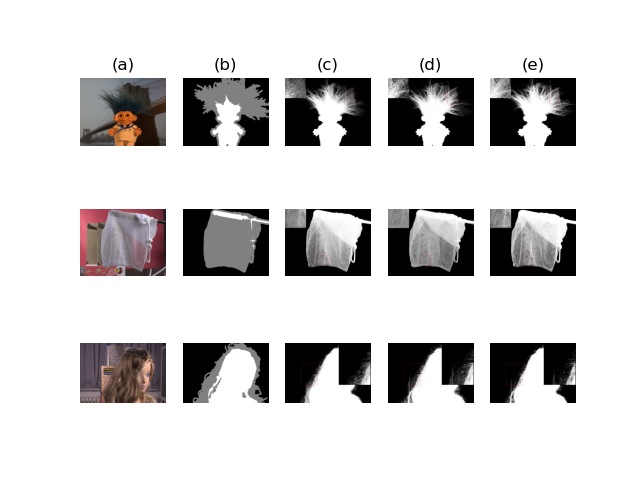
\includegraphics[]{bilder/result_comparison}
	\caption{Matting results for test images: (a) original images, (b) Trimaps (c) CFM algorithm, (d) KNNM algorithm, (e) LNCLM algorithm.}\label{fig_6}
\end{figure}

In Figure \ref{fig_6}, we can see that KNNM has harder segmentations and LNCLM is closer to the ground truth because of the combined local and NN color line models and the lack of smoothness assumption in KNNM. We also see that LNCLM better determines holes and complex regions due to its non local principle\cite{lnclm}. 

\begin{table}
	\centering
	\begin{tabular}{ c c c c c }
		\hline
		& CFM & KNN	& NNCLM & LNCLM \\ 
		\hline
		MSE & $2.18 * 10^{-2}$ & $2.44 * 10^{-2}$ & $2.12 * 10^{-2}$ & $1.81 * 10^{-2}$ \\  
		\hline
		SAD & $5.32 * 10^{3}$ & $6.11 * 10^{3}$	& $5.22 * 10^{3}$ & $4.78 * 10^{3}$ \\  
		\hline
	\end{tabular}
	\caption{MSE and SAD of our matting results.} \label{table:1}
\end{table}

A quantitative comparison \ref{table:1} shows that LNCLM outperformance KNNM and CFM in SAD and MSE. The reason is that LNCLM combines the strengths of both CFM and KNNM, giving us $\alpha$-mattes that cancel out each weakness. 

\begin{table}
	\centering
	\begin{tabular}{ c c c c c }
		\hline
		& CFM & KNN	& NNCLM		& LNCLM \\ 
		\hline
		MSE & $2.18 * 10^{-2}$ & $2.44 * 10^{-2}$	& $1.97 * 10^{-2}$ & $1.75 * 10^{-2}$ \\  
		\hline
		SAD & $5.32 * 10^{3}$ & $6.11 * 10^{3}$	& $5.00 * 10^{3}$ & $4.75 * 10^{3}$ \\  
		\hline
	\end{tabular}
	\caption{MSE and SAD of the matting results from the paper.}\label{table:2}
\end{table}

However, if we compare our MSE and SAD values to the values portrayed in table \ref{table:2} by the paper \cite{lnclm} and also compared to the alpha mattes shown on \cite{benchmark}, we see that our implementation is not as good as theirs. Figure 8 and table 2 shows the differences. 

\begin{figure}[htb]
	\begin{center}
		\includegraphics[width=350pt]{bilder/figure_7}
		\caption{Comparison between our implementation and the paper implementation}\label{fig_7}
	\end{center}
\end{figure}

We see that the CFM gives us the same MSE as well as SAD but a different MSE and SAD when it comes to the NNCLM, which means that the problem lies in the NNCLM. Furthermore, because we use the Algorithm part (\ref{laplace}) to calculate the Laplacian matrix both with neighbors of neighborscf and neighborsnnclm, it can not contain the problem because our values for CFM are correct. Therefore, the problem needs to lay in \ref{neighborsnnclm}. To solve this issue, we tried to change the parameters. First we tackled dws from the feature vector. We made the spatial coordinates more and less critical and concluded that a dws of \(0.6\) gave us the \(\alpha\) mattes nearest to the paper \cite{lnclm}. Secondly, we tried changing \(K\) in an attempt to place a more significant or lesser emphasis on the nonlocal principle. After testing different values for \(K\), we concluded that the preconditioned \(K\) is already the best. Last but not least, we also tried using KNNM instead of NNCLM for no particular reason, which did not help. 





\section{Conclusion}
We introduced and evaluated an enhanced image matting algorithm using local and non-local neighbors. Our suggested algorithm, LNCLM, overcomes the drawbacks of earlier techniques such as KNN-Matting (KNNM) and Closed-Form-Matting (CFM) by combining the advantages of the local color line model and the Nearest-Neighbors color line model.
We aimed to overcome problems like over-smoothing hole regions, correctly identifying complex regions, and being more precise in foreground segmentation. 
We conducted on 27 training images with ground truth and 8 images without ground truth and we found out that LNCLM outperforms KNNM and CFM both in MSE and SAD. We improved performance due to combining the strengths of local and non-local approaches.
The current implementation shows promising results and future work could focus on refining the parameters and enhancing the computational efficiency. We aim for performance comparable to state-of-the-art implementations.



